\documentclass[conference,10pt]{IEEEtran}
\IEEEoverridecommandlockouts

\usepackage[T1]{fontenc}
\usepackage{amsmath,amssymb}
\usepackage{graphicx}
\usepackage{booktabs,tabularx,array}
\usepackage[table]{xcolor}
\usepackage{cite}
\usepackage[expansion=false]{microtype}
\usepackage{tikz}
\usepackage[hidelinks]{hyperref}
\usepackage{url}
\usepackage{balance}
% Shared TikZ look for every diagram in the report: soft fills, rounded corners,
% blurred drop shadows, one sans-serif face — a clean "diagram tool" finish.
\usetikzlibrary{arrows.meta,shadows.blur,shapes.geometric,shapes.symbols,fit,backgrounds,positioning,calc}

\definecolor{inkD}{HTML}{1F2937}
\definecolor{inkM}{HTML}{4B5563}
\definecolor{inkL}{HTML}{6B7280}
\definecolor{appF}{HTML}{EEF2FF}\definecolor{appS}{HTML}{4F46E5}
\definecolor{modF}{HTML}{FFFFFF}\definecolor{modS}{HTML}{818CF8}
\definecolor{dbF}{HTML}{ECFDF5}\definecolor{dbS}{HTML}{059669}
\definecolor{wkF}{HTML}{F5F3FF}\definecolor{wkS}{HTML}{7C3AED}
\definecolor{exF}{HTML}{FFF7ED}\definecolor{exS}{HTML}{EA580C}
\definecolor{uiF}{HTML}{F0F9FF}\definecolor{uiS}{HTML}{0284C7}
\definecolor{secF}{HTML}{FEF2F2}\definecolor{secS}{HTML}{DC2626}
\definecolor{bndS}{HTML}{94A3B8}
\definecolor{flow}{HTML}{475569}

\tikzset{
  font=\sffamily\scriptsize, >={Stealth[length=2.2mm,width=1.6mm]},
  card/.style={rounded corners=2.5pt, line width=0.6pt, align=center, inner sep=4pt,
               blur shadow={shadow blur steps=6, shadow xshift=0.35mm, shadow yshift=-0.45mm, shadow opacity=22}},
  app/.style={card, draw=appS, fill=appF},
  mod/.style={card, draw=modS, fill=modF, minimum width=2.55cm, minimum height=1.02cm, text width=2.4cm},
  ext/.style={card, draw=exS, fill=exF, minimum width=3.0cm, minimum height=1.25cm, text width=2.85cm},
  ui/.style={card, draw=uiS, fill=uiF, minimum width=3.0cm, minimum height=1.25cm, text width=2.85cm},
  wk/.style={card, draw=wkS, fill=wkF, minimum width=2.75cm, minimum height=1.15cm, text width=2.6cm},
  sec/.style={card, draw=secS, fill=secF, minimum height=0.55cm},
  db/.style={cylinder, shape border rotate=90, aspect=0.16, draw=dbS, fill=dbF, line width=0.6pt, align=center,
             blur shadow={shadow blur steps=6, shadow xshift=0.35mm, shadow yshift=-0.45mm, shadow opacity=22}},
  ttl/.style={font=\sffamily\bfseries\scriptsize, text=inkD},
  sub/.style={font=\sffamily\tiny, text=inkM},
  lbl/.style={font=\sffamily\tiny, text=inkM, fill=white, fill opacity=0.92, text opacity=1, inner sep=1.2pt, rounded corners=1pt},
  arr/.style={->, draw=flow, line width=0.75pt, rounded corners=3pt},
  arr2/.style={<->, draw=flow, line width=0.75pt, rounded corners=3pt},
  rdash/.style={->, draw=flow, line width=0.7pt, dashed, dash pattern=on 2.5pt off 1.5pt, rounded corners=3pt},
  boundary/.style={draw=bndS, line width=0.8pt, dash pattern=on 4pt off 2.5pt, rounded corners=6pt},
  zonelbl/.style={font=\sffamily\bfseries\tiny, text=inkL, fill=white, inner sep=2pt},
  badge/.style={circle, fill=#1, text=white, font=\sffamily\bfseries\tiny, inner sep=0.8pt, minimum size=3.4mm},
}

% A small person glyph: \person{name}{x,y}{label}
\newcommand{\person}[3]{%
  \begin{scope}[shift={(#2)}]
    \fill[uiS!85] (0,0.26) circle (0.11);
    \fill[uiS!85] (-0.19,-0.02) .. controls (-0.19,0.14) and (0.19,0.14) .. (0.19,-0.02) -- cycle;
    \node[sub, anchor=north] (#1) at (0,-0.04) {#3};
  \end{scope}}


\newcolumntype{L}{>{\raggedright\arraybackslash}X}
\newcommand{\tbl}{\scriptsize\renewcommand{\arraystretch}{1.12}}

\begin{document}

\title{Project Proposal --- WalletWatch:\\An Assured, Near-Real-Time AML Monitoring System\\for Mobile Wallets}

\author{\IEEEauthorblockN{Hafiz Farhad Ahmed (22K-4787)}
\IEEEauthorblockA{Information Assurance --- Course Project\\
Department of Computer Science, FAST-NUCES Karachi\\
Instructor: Ali Naseer}}

\maketitle

\begin{abstract}
We propose to build and assess \emph{WalletWatch}, a working anti-money-laundering (AML) transaction
monitoring system for a synthetic Pakistani mobile wallet. The system will detect common laundering
typologies in near real time and give compliance staff a secure investigation and reporting
workflow. Unusually for detection projects, the monitoring system will itself be treated as the
asset to be assured: we will apply least privilege, role-based access control, separation of
duties, data masking and tamper-evident logging, map them to ISO/IEC 27001 and NIST standards,
assess risk following ISO 31000 and NIST SP 800-30 (including cyber insurance as risk transfer), and
design a Security Education, Training and Awareness (SETA) programme for its users.
\end{abstract}

\section{Background and Motivation}
Mobile wallets let money move instantly and cheaply through agents and person-to-person transfers,
which also makes them attractive for laundering criminal proceeds~\cite{fatf2013npps}. Pakistani
reporting entities must monitor transactions and file Suspicious Transaction Reports with the
Financial Monitoring Unit through goAML~\cite{amla2010,fmu2021ctr}. Rule-based monitoring is known to
produce very high false-positive rates~\cite{deloitte2020tm}, and the monitoring system concentrates
sensitive identity data and legally significant decisions. An insider who can suppress alerts,
approve their own report or alter the audit trail undermines the whole control.

\section{Problem Statement}
How can a mobile-wallet operator detect laundering patterns in near real time \emph{and} demonstrate
justified confidence that the monitoring system itself preserves the confidentiality, integrity and
availability of its data and decisions?

\section{Objectives}
\begin{enumerate}
  \item Build a synthetic wallet with planted laundering rings and benign look-alike behaviour,
        with full ground truth, following the AMLworld methodology~\cite{altman2023amlworld}.
  \item Detect at least five laundering typologies in near real time, combining rules, temporal
        graph analysis and one explainable ML model~\cite{chen2016xgboost,lundberg2017shap}.
  \item Provide an alert $\rightarrow$ case $\rightarrow$ STR workflow with maker--checker approval.
  \item Implement and test IA controls: RBAC, least-privilege database roles, PII masking and a
        tamper-evident audit log~\cite{sandhu1996rbac,clarkwilson1987,schneier1999audit}.
  \item Produce an assurance case, a standards mapping (ISO/IEC 27001:2022, NIST SP 800-53 r5,
        CSF 2.0), a risk register with treatment, and a SETA programme.
  \item Measure detection quality (precision, recall, time to detect) honestly against ground truth.
\end{enumerate}

\section{Scope}
\textbf{In scope:} the synthetic data generator, the monitoring pipeline, the analyst dashboard,
security controls, automated tests, and the written assessment and presentation.
\textbf{Out of scope:} customer-side fraud (account takeover, SIM swap), sanctions screening, goAML
XML submission, TLS and single sign-on, and any real customer data.

\section{Proposed Approach}

\begin{figure}[t]
  \centering
  \resizebox{\columnwidth}{!}{% System architecture (Fig. 1). Coordinates in cm; scaled to \textwidth by the caller.
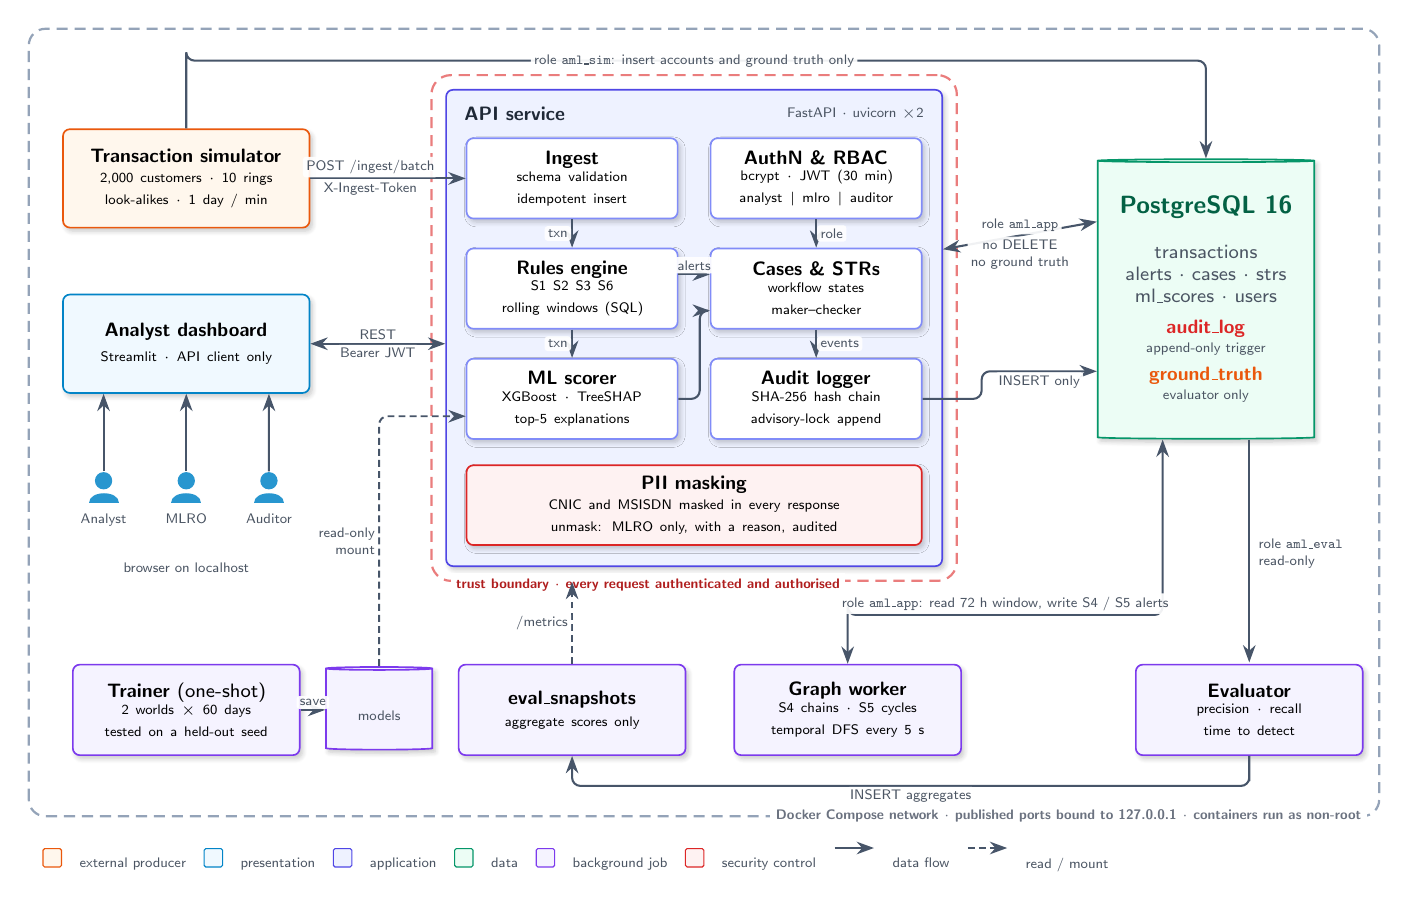
\begin{tikzpicture}[x=1cm,y=1cm]

% ---------------------------------------------------------------- producers and users
\node[ext] (sim)  at (1.6,5.15) {\textbf{Transaction simulator}\\[1pt]{\tiny 2,000 customers $\cdot$ 10 rings\\look-alikes $\cdot$ 1 day / min}};
\node[ui]  (dash) at (1.6,3.05) {\textbf{Analyst dashboard}\\[1pt]{\tiny Streamlit $\cdot$ API client only}};
\person{pA}{0.55,1.05}{Analyst}
\person{pM}{1.6,1.05}{MLRO}
\person{pU}{2.65,1.05}{Auditor}
\foreach \p/\dx in {pA/-1.05, pM/0, pU/1.05}
  \draw[arr] ($(\p.north)+(0,0.42)$) -- ($(dash.south)+(\dx,0)$);
\node[sub] at (1.6,0.2) {browser on localhost};

% ---------------------------------------------------------------- API service
\node[app, minimum width=6.3cm, minimum height=6.05cm] (api) at (8.05,3.25) {};
\node[ttl, anchor=north west] at ($(api.north west)+(0.12,-0.1)$) {API service};
\node[sub, anchor=north east] at ($(api.north east)+(-0.12,-0.12)$) {FastAPI $\cdot$ uvicorn $\times$2};

\node[mod] (ing)  at (6.5,5.15) {\textbf{Ingest}\\{\tiny schema validation\\idempotent insert}};
\node[mod] (auth) at (9.6,5.15) {\textbf{AuthN \& RBAC}\\{\tiny bcrypt $\cdot$ JWT (30 min)\\analyst $\mid$ mlro $\mid$ auditor}};
\node[mod] (rul)  at (6.5,3.75) {\textbf{Rules engine}\\{\tiny S1 S2 S3 S6\\rolling windows (SQL)}};
\node[mod] (case) at (9.6,3.75) {\textbf{Cases \& STRs}\\{\tiny workflow states\\maker--checker}};
\node[mod] (ml)   at (6.5,2.35) {\textbf{ML scorer}\\{\tiny XGBoost $\cdot$ TreeSHAP\\top-5 explanations}};
\node[mod] (aud)  at (9.6,2.35) {\textbf{Audit logger}\\{\tiny SHA-256 hash chain\\advisory-lock append}};
\node[sec, minimum width=5.65cm, text width=5.5cm] (mask) at (8.05,1.0)
      {\textbf{PII masking}\\[1pt]{\tiny CNIC and MSISDN masked in every response\\ unmask: MLRO only, with a reason, audited}};

\draw[arr] (ing) -- node[lbl, left] {txn} (rul);
\draw[arr] (rul) -- node[lbl, left] {txn} (ml);
\draw[arr] ($(rul.east)+(0,0.18)$) -- node[lbl, above] {alerts} ($(case.west)+(0,0.18)$);
\draw[arr] (ml.east) -- ++(0.27,0) |- ($(case.west)+(0,-0.28)$);
\draw[arr] (case) -- node[lbl, right] {events} (aud);
\draw[arr] (auth) -- node[lbl, right] {role} (case);

\node[fit=(api), inner sep=5pt, draw=secS!60, line width=0.8pt, dash pattern=on 4pt off 2.5pt, rounded corners=7pt] (tb) {};
\node[zonelbl, text=secS!80!black, anchor=north west] at ($(tb.south west)+(0.25,0.12)$) {trust boundary $\cdot$ every request authenticated and authorised};

% ---------------------------------------------------------------- data tier
\node[db, minimum width=2.75cm, minimum height=3.55cm] (pg) at (14.55,3.6) {};
\node[ttl, text=dbS!65!black, font=\sffamily\bfseries\small] at ($(pg.north)+(0,-0.62)$) {PostgreSQL 16};
\node[font=\sffamily\scriptsize, text=inkM, align=center, anchor=north] at ($(pg.north)+(0,-0.98)$) {%
  transactions\\ alerts $\cdot$ cases $\cdot$ strs\\ ml\_scores $\cdot$ users\\[3pt]
  {\color{secS}\textbf{audit\_log}}\\[-1pt]{\tiny append-only trigger}\\[2pt]
  {\color{exS}\textbf{ground\_truth}}\\[-1pt]{\tiny evaluator only}};

% ---------------------------------------------------------------- background jobs
\node[wk] (tr)   at (1.6,-1.6)   {\textbf{Trainer} (one-shot)\\{\tiny 2 worlds $\times$ 60 days\\tested on a held-out seed}};
\node[db, minimum width=1.35cm, minimum height=1.05cm, draw=wkS, fill=wkF] (vol) at (4.05,-1.6) {};
\node[sub] at ($(vol.center)+(0,-0.07)$) {models};
\node[wk] (snap) at (6.5,-1.6)   {\textbf{eval\_snapshots}\\{\tiny aggregate scores only}};
\node[wk] (gw)   at (10.0,-1.6)  {\textbf{Graph worker}\\{\tiny S4 chains $\cdot$ S5 cycles\\temporal DFS every 5 s}};
\node[wk] (ev)   at (15.1,-1.6)  {\textbf{Evaluator}\\{\tiny precision $\cdot$ recall\\time to detect}};

% ---------------------------------------------------------------- flows between tiers
\draw[arr] (sim.east) -- node[lbl, above] {POST /ingest/batch} node[lbl, below] {X-Ingest-Token} (sim.east -| tb.west) -- (ing.west);
\draw[arr] (sim.north) |- ++(0,0.86) -| (pg.north);
\node[lbl] at (8.05,6.64) {role \texttt{aml\_sim}: insert accounts and ground truth only};
\draw[arr2] (dash.east) -- node[lbl, above] {REST} node[lbl, below] {Bearer JWT} (dash.east -| api.west);
\draw[arr2] ($(api.east)+(0,1.0)$) -- node[lbl, above] {role \texttt{aml\_app}} node[lbl, below, align=center] {no DELETE\\no ground truth} ($(pg.west)+(0,1.0)$);
\draw[arr] (aud.east) -- ++(0.75,0) |- node[lbl, pos=0.75, below] {INSERT only} ($(pg.west)+(0,-0.9)$);
\draw[arr2] (gw.north) |- ++(0,0.62) -| node[lbl, pos=0.25, above] {role \texttt{aml\_app}: read 72 h window, write S4 / S5 alerts} ($(pg.south)+(-0.55,0)$);
\draw[arr] ($(pg.south)+(0.55,0)$) -- ($(pg.south)+(0.55,-2.83)$);
\node[lbl, anchor=west, align=left] at ($(pg.south)+(0.62,-1.45)$) {role \texttt{aml\_eval}\\read-only};
\draw[arr] (ev.south) |- ++(0,-0.38) -| node[lbl, pos=0.25, below] {INSERT aggregates} (snap.south);
\draw[rdash] (snap.north) -- node[lbl, left] {/metrics} (snap.north |- tb.south);
\draw[arr] (tr.east) -- node[lbl, above] {save} (vol.west);
\draw[rdash] (vol.north) |- node[lbl, pos=0.25, left, align=right] {read-only\\mount} ($(ml.south west)+(0,0.3)$);

% ---------------------------------------------------------------- outer boundary + legend
\begin{scope}[on background layer]
  \draw[boundary] (-0.4,-2.95) rectangle (16.75,7.05);
\end{scope}
\node[zonelbl, anchor=east] at (16.6,-2.95) {Docker Compose network $\cdot$ published ports bound to 127.0.0.1 $\cdot$ containers run as non-root};

\matrix[anchor=north west, column sep=3pt, font=\sffamily\tiny, text=inkM] at (-0.35,-3.15) {
  \node[fill=exF, draw=exS, minimum size=2.2mm, rounded corners=0.6pt]{}; & \node{external producer}; &
  \node[fill=uiF, draw=uiS, minimum size=2.2mm, rounded corners=0.6pt]{}; & \node{presentation}; &
  \node[fill=appF, draw=appS, minimum size=2.2mm, rounded corners=0.6pt]{}; & \node{application}; &
  \node[fill=dbF, draw=dbS, minimum size=2.2mm, rounded corners=0.6pt]{}; & \node{data}; &
  \node[fill=wkF, draw=wkS, minimum size=2.2mm, rounded corners=0.6pt]{}; & \node{background job}; &
  \node[fill=secF, draw=secS, minimum size=2.2mm, rounded corners=0.6pt]{}; & \node{security control}; &
  \draw[arr] (0,0) -- (0.5,0); & \node{data flow}; &
  \draw[rdash] (0,0) -- (0.5,0); & \node{read / mount}; \\
};
\end{tikzpicture}
}
  \caption{Planned architecture: producer, API trust boundary, data tier with least-privilege roles,
  background jobs.}
  \label{fig:arch}
\end{figure}

The planned architecture (Fig.~\ref{fig:arch}) is a set of containers started with one command.
A simulator streams transactions to a FastAPI service that validates and stores them, evaluates
typology rules over rolling windows, and scores them with an XGBoost model explained by TreeSHAP. A
graph worker searches for time-ordered layering chains and round-trips. A Streamlit dashboard,
which talks only to the API, serves three roles: analyst, Money Laundering Reporting Officer (MLRO)
and auditor. A separate evaluator, under a read-only database role, compares alerts with ground
truth, so the detector never sees the answers.

\section{Information Assurance Considerations}

\begin{table}[t]
\caption{Planned controls and the standards they address}\label{tab:plan}
\centering\tbl
\begin{tabularx}{\columnwidth}{@{}Lll@{}}
\toprule
Control & ISO 27001 A. & NIST 800-53 \\ \midrule
Role-based access control & 5.15, 5.18 & AC-2, AC-3 \\
Maker--checker STR approval & 5.3 & AC-5 \\
Least-privilege DB roles & 8.2 & AC-6 \\
Password hashing, signed tokens & 8.5 & IA-2, IA-5 \\
PII masking, audited unmask & 8.11, 5.34 & AC-3, SI-19 \\
Tamper-evident audit log & 8.15 & AU-9, AU-10 \\
Automated security tests & 8.29 & SA-11 \\
SETA programme & 6.3 & AT-2, AT-3 \\
\bottomrule
\end{tabularx}
\end{table}

\textbf{Controls.} Table~\ref{tab:plan} lists the planned controls, mapped to ISO/IEC 27001:2022
Annex A~\cite{iso27001} and NIST SP 800-53 Rev.~5~\cite{nist80053}.

\textbf{Risk.} We will identify assets and threats, rate inherent and residual risk on 5$\times$5
scales (NIST SP 800-30~\cite{nist80030}), and choose a treatment for each risk (avoid, mitigate,
transfer or accept) following ISO 31000 and ISO/IEC 27005~\cite{iso31000,iso27005}. That includes
whether cyber insurance can transfer part of the financial impact~\cite{romanosky2019insurance}.

\textbf{Assurance.} Each security claim will be backed by an automated test, forming an assurance
case of claims, arguments and evidence.

\textbf{People.} A SETA programme following NIST SP 800-50 Rev.~1~\cite{nist80050r1} and Whitman and
Mattord~\cite{whitman2012principles} will cover agents, analysts, MLROs and auditors.

\section{Evaluation Plan}
\begin{itemize}
  \item \textbf{ML:} PR-AUC, precision and recall on a held-out synthetic world with a different
        random seed.
  \item \textbf{System:} account-level precision and recall per scenario and typology, time to
        detect per ring, and the number of benign look-alikes flagged.
  \item \textbf{Security:} automated tests that attempt each violation, such as a forged token, a
        cross-role action, self-approval, reading ground truth, and editing the audit log.
\end{itemize}

\section{Deliverables}
(1) Source code with Docker Compose deployment and test suite; (2) a working live demonstration;
(3) the project report with architecture, assessment, standards mapping, risk register and SETA
programme; (4) presentation slides; (5) a viva demonstration script.

\section{Work Plan}

\begin{table}[t]
\caption{Work plan}\label{tab:plan2}
\centering\tbl
\begin{tabularx}{\columnwidth}{@{}lLl@{}}
\toprule
Phase & Work & Exit criterion \\ \midrule
0 & Skeleton, schema, DB roles & stack starts; schema applied \\
1 & Simulator, look-alikes, ground truth & 60-day dataset generated \\
2 & Ingest and rules (S1, S2, S3, S6) & alerts with frozen evidence \\
3 & Security: auth, RBAC, masking, audit chain & security tests pass \\
4 & Graph worker (S4, S5) & planted rings detected \\
5 & Dashboard, cases, STR workflow & full flow clickable \\
6 & ML model with explanations & held-out PR-AUC reported \\
7 & Evaluation, report, slides & deliverables complete \\
\bottomrule
\end{tabularx}
\end{table}

Table~\ref{tab:plan2} lists the phases. Each phase ends with a demonstrable exit criterion.

\section{Project Risks}
\textbf{Scope creep}: mitigated by a written specification with explicit core and stretch features.
\textbf{Circular evaluation} on synthetic data: mitigated by benign look-alikes, a held-out seed and
open reporting of false positives.
\textbf{Unfamiliar AML domain}: mitigated by grounding typologies in FATF and FMU
guidance~\cite{fatf2012rec,fatf2018pml}.

\section{Ethics and Data}
Only synthetic data will be used; no real customer, CNIC or phone data is processed. The system is a
training artefact and produces no reports to any authority.

\balance
\bibliographystyle{ieeetr}
\bibliography{refs}

\end{document}
